%\begin{equation}
%f_i^{(j,~k)} = \dfrac{\mathbb{E}_i^{(j,~k)}}{\mathbb{E}_i^{(k)}}
%\end{equation}
%de lo cual se deriva que:
%\begin{equation}
%f^{(j,~k)} = \sum_i f_i^{(j,~k)}, ~~~~ f_i^{(k)} = \sum_j f_i^{(j,~k)} ~~~~ y ~~~~~ f^{(k)} = \sum_{ij} f_i^{(j,~k)}
%\end{equation}

Procesando la información relevante a la investigación se hace necesario identificar los eventos a los que se les dedicará el estudio, conocer la frecuencia de la cantidad de muones por eventos $\mathbb{E}_i^{(j,~\mathtt{k})}$ para los muones reconstruidos por los detectores en las configuraciones \texttt{CMS} (correspondiente a Run-2) y \texttt{HL} (Alta Luminosidad) es el primer paso en la investigación.

\begin{figure}[h!]
\centering
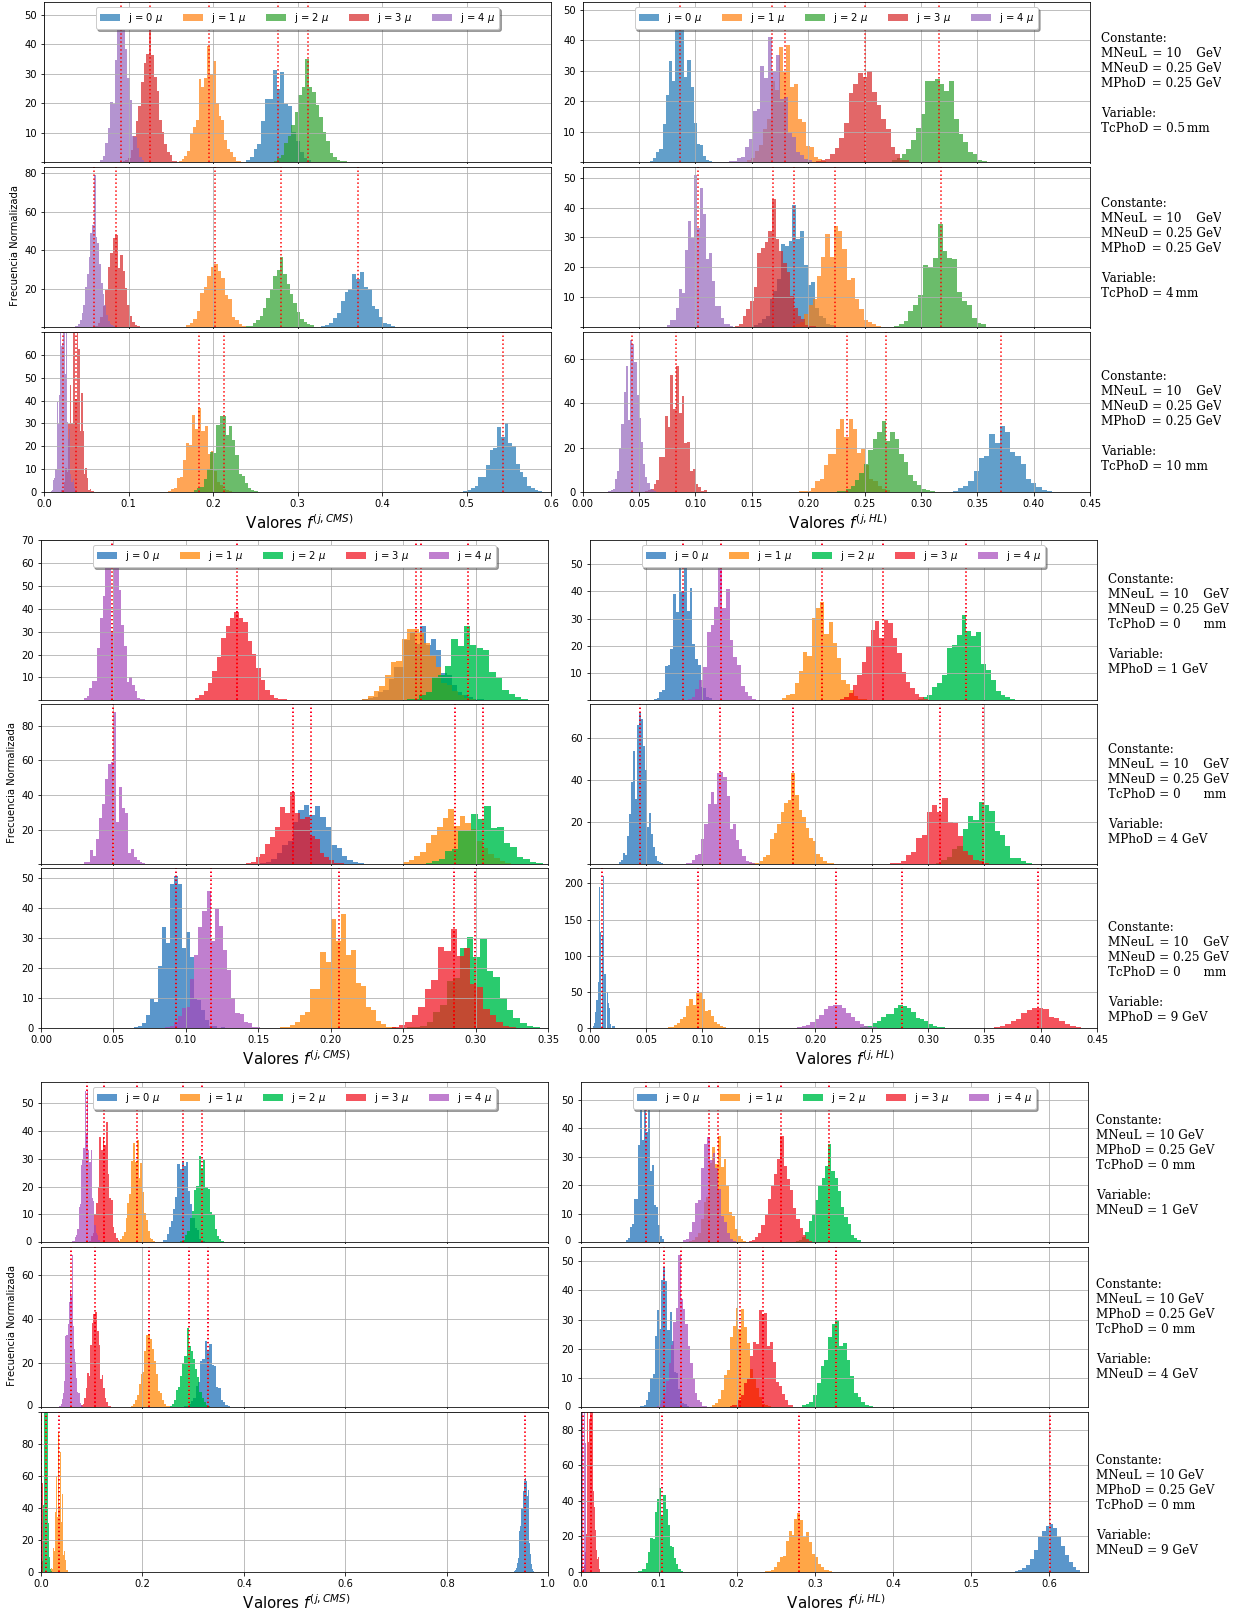
\includegraphics[width=.92\textwidth]{Simulacion/imagenes/Distribucion_EntriesALL.png}
\caption{Distribuciones de frecuencia de las entradas $f^{(j,~k)}$ ante cambios de \texttt{TcPhoD}, \texttt{MPhoD} y  \texttt{MNeuD}.}
\label{entradas}
\end{figure}


Las Figs. \ref{entradas} %, \ref{entradas2} y \ref{entradas3} 
muestran las histogramas normalizados de los porcentajes de eventos con diferentes contenidos muónicos, estos son comparados ante el cambio de los parámetros \texttt{TcPhoD}, \texttt{MPhoD} y \texttt{MMeuD} respectivamente. En estos gráficos se puede observar la alta dependencia entre los valores normalizados de $\mathbb{E}^{(j,~\mathtt{k})}$ sobre los eventos totales (\texttt{Event}$= 10~000$), y como estos varian con respecto a los parámetros de generación, identificar esta dependencia se hace necesaria por motivos de caracterización y generalización.

\subsubsection{Error en la elección de muestra.}
Si consideramos que la forma de estas distribuciones corresponde con una gaussiana, el error en la frecuencia es calculable:
\begin{equation}\label{error0}
\dfrac{\Delta \mathbb{E}^{(j,~\mathtt{k})}}{\mathbb{E}^{(j,~\mathtt{k})}} = Z_{\frac{\alpha}{2}} \sqrt{\dfrac{p(1-p)}{\mathbb{E}^{(j,~\mathtt{k})}}} 
\end{equation}%\sqrt{\dfrac{\mathbb{E}^{(\mathtt{k})}- \mathbb{E}^{(j,~\mathtt{k})}}{\mathbb{E}^{(\mathtt{k})}-1}}
donde:\\
\begin{tabular}{lp{14cm}}
$Z_{\frac{\alpha}{2}}$ & es un parámetro que depende del nivel de confianza $(1-\alpha$). Algunos de los valores mas usados son: $Z_{\frac{0.1}{2}}=1.65$, $Z_{\frac{0.05}{2}}=1.96$ y $Z_{\frac{0.01}{2}}=2.58$.\\
$p$ & es la probabilidad ocurrencia, ya que no se conoce se toma el valor máximo posible de $p_{max}=0.5$.
\end{tabular}

Para realizar los análisis lo más general posible se denota una frecuencia adsoluta o porcentual como:
\begin{equation}
f^{(j,~k)} = \dfrac{\mathbb{E}^{(j,~k)}}{\mathbb{E}^{(k)}}
\end{equation}
donde al sustituir en la ec. \ref{error0}, tenemos:
\begin{equation}
\dfrac{\Delta f^{(j,~\mathtt{k})}}{f^{(j,~\mathtt{k})}} = Z_{\frac{\alpha}{2}} \sqrt{\dfrac{p(1-p)}{f^{(j,~\mathtt{k})} \cdot \mathbb{E}^{(\mathtt{k})}}} 
\end{equation}
%\end{landscape} \end{landscape}
\subsubsection{Probabilidad de ocurrencia.}

Para cierta combinación de parámetros, los detectores en sus diferentes configuraciones tienen una probabilidad $p$ de ocurrencia o reconstrucción del muón, si se hace la suposición de que esta probabilidad es fija para cierta morfologia en las propiedades de los muones entonces podemos hacer uso de la binomial para facilitar las comparaciones entre los eventos.
Partiendo de la ecuación binomial:
\begin{equation}\label{binomial}
f^{(j,~k)} = \dfrac{n_{max}!}{n_j!~(n_{max} - n_j)!} ~ p^{n_j} ~ (1-p)^{n_{max}-n_j}
\end{equation}
donde:\\
\begin{tabular}{lp{14cm}}
$n_{j} = j$ & número de muones. Para nuestras muestras los valores admisibles son $j = \{0,~1,~2,~3,~4\}$, resultado de lo cual $n_{max} = n_{4\mu} = 4$. \\
$p$ & es la probabilidad ocurrencia o reconstrucción de los muones.
\end{tabular}
Dado que el $\backsim 80\%$ de los datos generados a los que se tiene acceso solo se posee información de los eventos $\mathbb{E}^{(4\mu,~\mathtt{k})}$, entonces podemos calcular la probabilidad de ocurrencia como:
\begin{equation}\label{ocurrencia}
f^{(4\mu,~k)} = \dfrac{4!}{4!~0!} ~ p^{4} ~ (1-p)^{0} = p^{4} ~~~\Rightarrow ~~~ p = \sqrt[4]{f^{(4\mu,~k)}}
\end{equation}

Finalmente sustituyendo la ec. \ref{ocurrencia} en ec. \ref{binomial} tenemos:
\begin{equation}\label{binomialF}
f^{(j,~k)} = \dfrac{n_{max}!}{n_j!~(n_{max} - n_j)!} ~ (f^{(4\mu,~k)})^{\frac{n_j}{4}} ~ (1-(f^{(4\mu,~k)})^{\frac{1}{4}})^{n_{max}-n_j}
\end{equation}
Con esta ecuación se podrá simular los valores $f^{(j,~k)}$ para los datos con información reducida, aunque dada las suposiciones que deriban de esta ecuación los errores observados de la comparación con los datos reales pueden llegar a $20\%
,$.%$\Delta f^{(j,~k)} / f^{(j,~k)} = 20\%$ 



\subsubsection{Correspondencia entre los eventos de interés y los parámetros de generación.}

Algunos ejemplos de estos resultados de valores de $f^{(0\mu,~k)} $ y $f^{(4\mu,~k)} $ los podremos observar en la Tabla \ref{Numero_de_Entradas} y en los gráficos de la Fig. \ref{entradasALL}. En estos se puede observar una clara tendencia en la frecuencia de casos $f^{(j,~k)} $, en general se puede constatar la disminución de eventos de interés con el aumento del tiempo de vida del fotón  (\texttt{TcPhoD}) y de la masa del neutralino oscuro (\texttt{MNeuD}), en contraste se registra aumento de los eventos de interés con la masa del fotón oscuro, en el caso de cambios de la masa del neutralino ligero (\texttt{MNeuL}) los datos muestran variaciones pequeñas en el rango definido por lo que la existencia de una tendencia no es posible corroborar en el grupo de datos simulados.

% Al comparar los resultados podemos observar empíricamente una tendencia de estos valores de frecuencia ante cambios de los parámetros de generación.

%\begin{landscape}
\begin{table}
\begin{scriptsize}
\begin{tabular}{|cccccccc|}
\hline
$\texttt{MNeuL}$ & $\texttt{MNeuD}$ & $\texttt{MPhoD}$ & $\texttt{TcPhoD}$ & $f^{(0\mu,~\texttt{CMS})}$ & $f^{(0\mu,~\texttt{HL})}$ & $f^{(4\mu,~\texttt{CMS})}$ & $f^{(4\mu,~\texttt{HL})}$ \\
$\texttt{(GeV)}$ & $\texttt{(GeV)}$ & $\texttt{(GeV)}$ & $\texttt{(mm)}$ & & & & \\
\hline
10 & 0.25 & 0.25 & 0.5 & 0.2777 $\pm$ 0.0068 & 0.0864 $\pm$ 0.0038 & 0.0920 $\pm$ 0.0040 & 0.1678 $\pm$ 0.0053\\
& & & 2 & 0.3040 $\pm$ 0.0071 & 0.1227 $\pm$ 0.0045 & 0.0779 $\pm$ 0.0036 & 0.1355 $\pm$ 0.0047 \\
& & & 4 & 0.3718 $\pm$ 0.0078 & 0.1872 $\pm$ 0.0056 & 0.0597 $\pm$ 0.0032 & 0.1024 $\pm$ 0.0041\\
& & & 10 & 0.5428 $\pm$ 0.0095 & 0.3710 $\pm$ 0.0079 & 0.0227 $\pm$ 0.0019 & 0.0433 $\pm$ 0.0027\\
& & & 50 & 0.8570 $\pm$ 0.0119 & 0.7568 $\pm$ 0.0112 & 0.0016 $\pm$ 0.0005 & 0.0039 $\pm$ 0.0008\\
& & & 100 & 0.9217 $\pm$ 0.0123 & 0.8664 $\pm$ 0.0120 & 0.0002 $\pm$ 0.0002 & 0.0006 $\pm$ 0.0003\\
\hline
%10 & 0.25 & 0.25 & 0 & 0.2744 $\pm$ 0.0410 & 0.0813 $\pm$ 0.0223 & 0.0881 $\pm$ 0.0232 & 0.1622 $\pm$ 0.0315 \\
10 & 0.25 & 2 & 0 & 0.2467 $\pm$ 0.0064 & 0.0699 $\pm$ 0.0034 & 0.0497 $\pm$ 0.0029 & 0.1135 $\pm$ 0.0043 \\
& & 4 & & 0.1862 $\pm$ 0.0055 & 0.0446 $\pm$ 0.0027 & 0.0494 $\pm$ 0.0029 & 0.1157 $\pm$ 0.0040 \\
& & 6 & & 0.1286 $\pm$ 0.0046 & 0.0253 $\pm$ 0.0021 & 0.0599 $\pm$ 0.0032 & 0.1456 $\pm$ 0.0049\\
& & 8 & & 0.0998 $\pm$ 0.0040 & 0.0134 $\pm$ 0.0015 & 0.0957 $\pm$ 0.0040 & 0.1960 $\pm$ 0.0057\\
\hline
10 & 2 & 0.25 & 0 & 0.2929 $\pm$ 0.0069 & 0.0890 $\pm$ 0.0038 & 0.0852 $\pm$ 0.0038 & 0.1604 $\pm$ 0.0052\\
& 4 & & & 0.3287 $\pm$ 0.0074 & 0.1072 $\pm$ 0.0042 & 0.0586 $\pm$ 0.0031 & 0.1281 $\pm$ 0.0046 \\
& 6 & & & 0.4265 $\pm$ 0.0084 & 0.1536 $\pm$ 0.0051 & 0.0221 $\pm$ 0.0019 & 0.0831 $\pm$ 0.0037\\
& 8 & & & 0.7097 $\pm$ 0.0108 & 0.3203 $\pm$ 0.0073 & 0.0022 $\pm$ 0.0006 & 0.0193 $\pm$ 0.0018\\
\hline
20 & 1 & 1 & 0 & -- & -- & 0.0560 $\pm$ 0.0030 & 0.1176 $\pm$ 0.0044 \\
30 & & & &  --  & -- & 0.0480 $\pm$ 0.0028 & 0.1224 $\pm$ 0.0045\\
40 & & & & -- & -- &  0.0524 $\pm$ 0.0030 &  0.1319 $\pm$ 0.0047 \\
50 & & & & -- & -- & 0.0583 $\pm$ 0.0031 & 0.1391 $\pm$ 0.0048 \\
\hline
\end{tabular}
\caption{Ejemplos de valores de frecuencia muónica para combinaciones de generación}
\label{Numero_de_Entradas}
\end{scriptsize}
\end{table}

\begin{figure}[h]
\centering
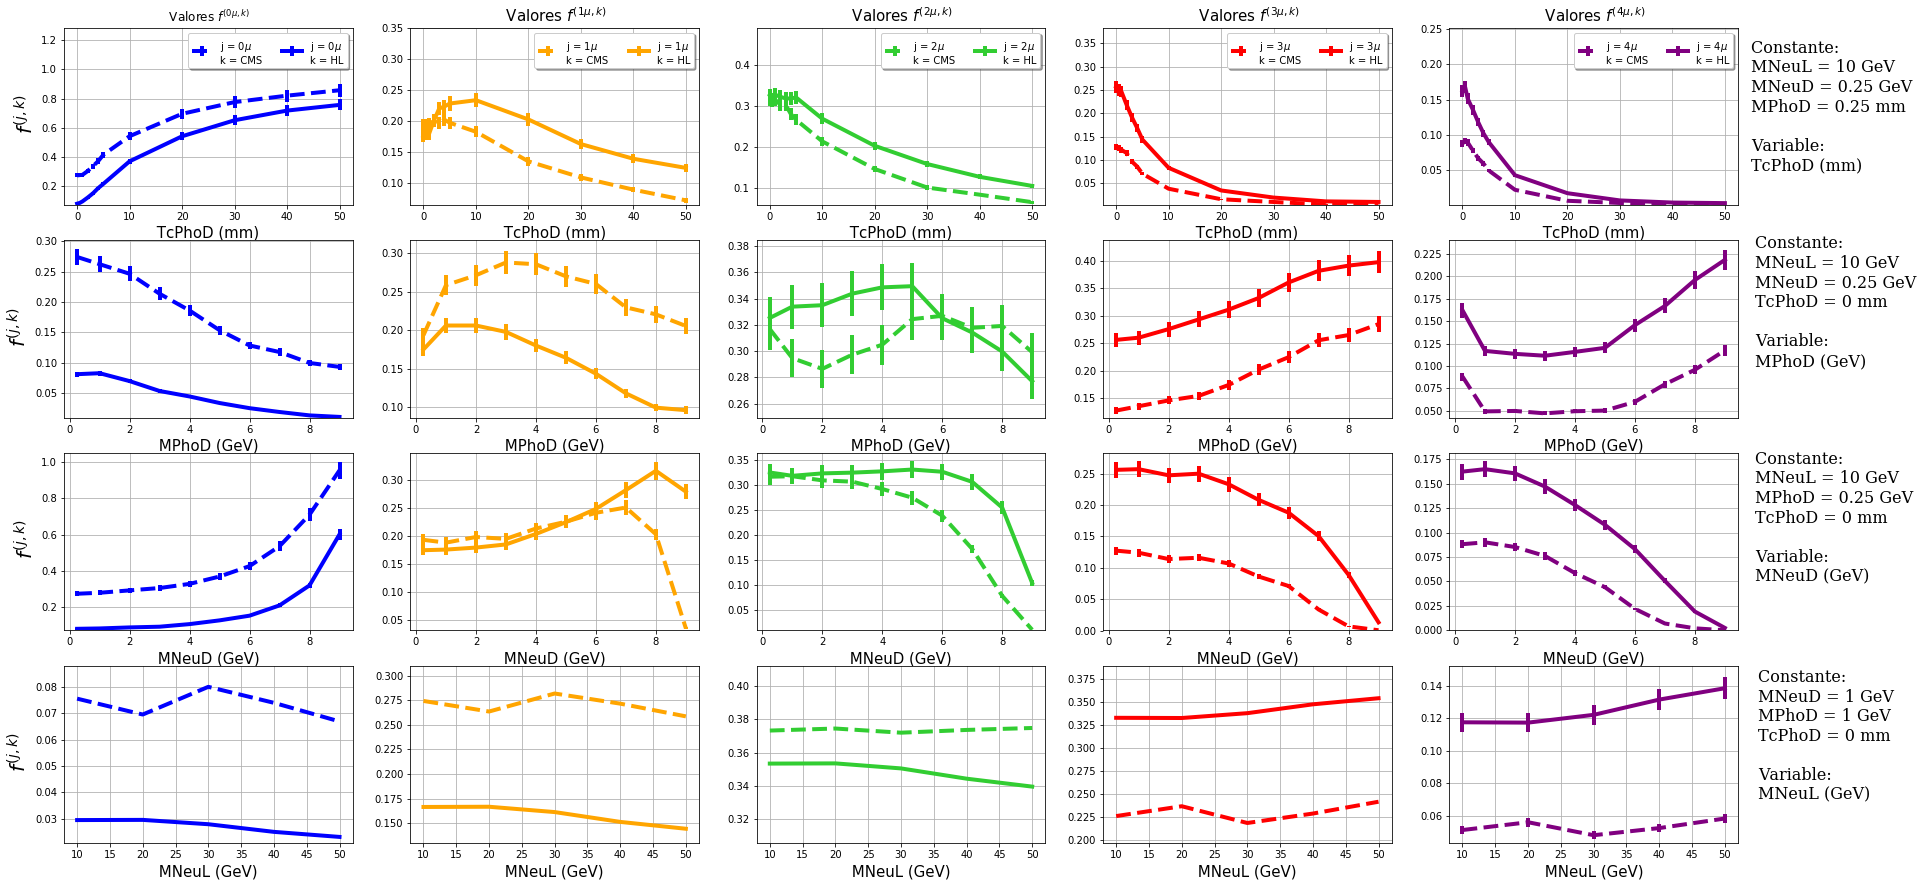
\includegraphics[width=.95\textwidth]{Simulacion/imagenes/Comparacion_Distribucion_Entries.png}
\caption{Distribuciones de frecuencia de las entradas $f^{(j,~k)}$ ante cambios de \texttt{MNeuD}.}
\label{entradasALL}
\end{figure}

\subsubsection{Regresión de datos de frecuencia $f^{(j,~k)}$.}

Con la intención de realizar una caracterización eficiente de la cantidad de eventos de interés y de su dependencia con los parámetros de generación, se intenta utilizar métodos simples de regresión para valorar la posibilidad de inferir información pertinente a la frecuencia de los eventos. Para esto se utilizán los métodos presentados ya en la seccion \ref{Cap_regresion} mediante una aproximación lineal como la propuesta en la ec. \ref{regresion} y con una red neuronal como la presentada en la Fig. \ref{neuronas}.

\begin{figure}[h]
\centering
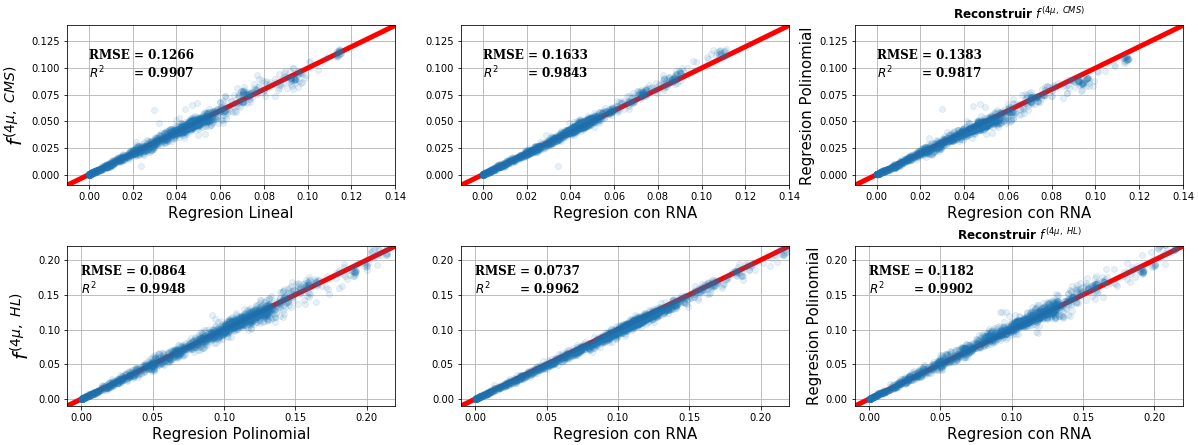
\includegraphics[width=1\textwidth]{Simulacion/imagenes/ML_Entries.png}
\caption{Resultados de la regresión de los valores de frecuencia $f^{(4\mu,~k)}$.}
\label{regresionALL}
\end{figure}


Al implementar el método de regresión polinomial sobre los datos $f^{(4\mu,~CMS)}$ y $f^{(4\mu,~HL)}$ considerando como valores independientes $x_i=\{$ \texttt{MMeuL}, \texttt{MMeuD}, \texttt{MPhoD}, \texttt{TcPhoD}$\}$ solo hasta el orden $k = 6$ se lográ encontrar una correspondencia entre los valores simulados y los predichos, siendo corrobarada por los parámetros de confianza \textbf{RMSE} y $\mathbf{R^2}$ con valores pequeños y cercanos a 1, respectivamente. 

Al realizar la regresión de las frecuencias $f^{(4\mu,~k)}$ haciendo uso del método \textbf{RNA} según una configuración semejante a la Fig. \ref{regresion} con $k=4$ capas ocultas con cantidad de nodos $m_k=\{9,~7,~5,~3\}$ por cada uno respectivamente, se obtuvo un modelo con valores de \textbf{RMSE} y $\mathbf{R^2}$ comparables con los del método de regresión lineal explicado con anterioridad.

En la Fig. \ref{neuronas} también se puede observar una comparación de los resultados de los dos métodos al intentar reconstruir la información de los valores de frecuencia $f^{(4\mu,~k)}$ mostrando una alta linealidad en los resultados obtenidos válidando su implementación como método de análisis. Al analizar los errores de estás predicciones con los datos originales se obtuvo que lo resultados diferencian hasta en un $\sim 30\%$, siendo una de las posibles consecuencias de estos altos errores el pequeño valor del parámetro de generación \texttt{Event} (ver sección \ref{Cap_genera}).

%\begin{landscape}
%\begin{figure}[h]
%\centering
%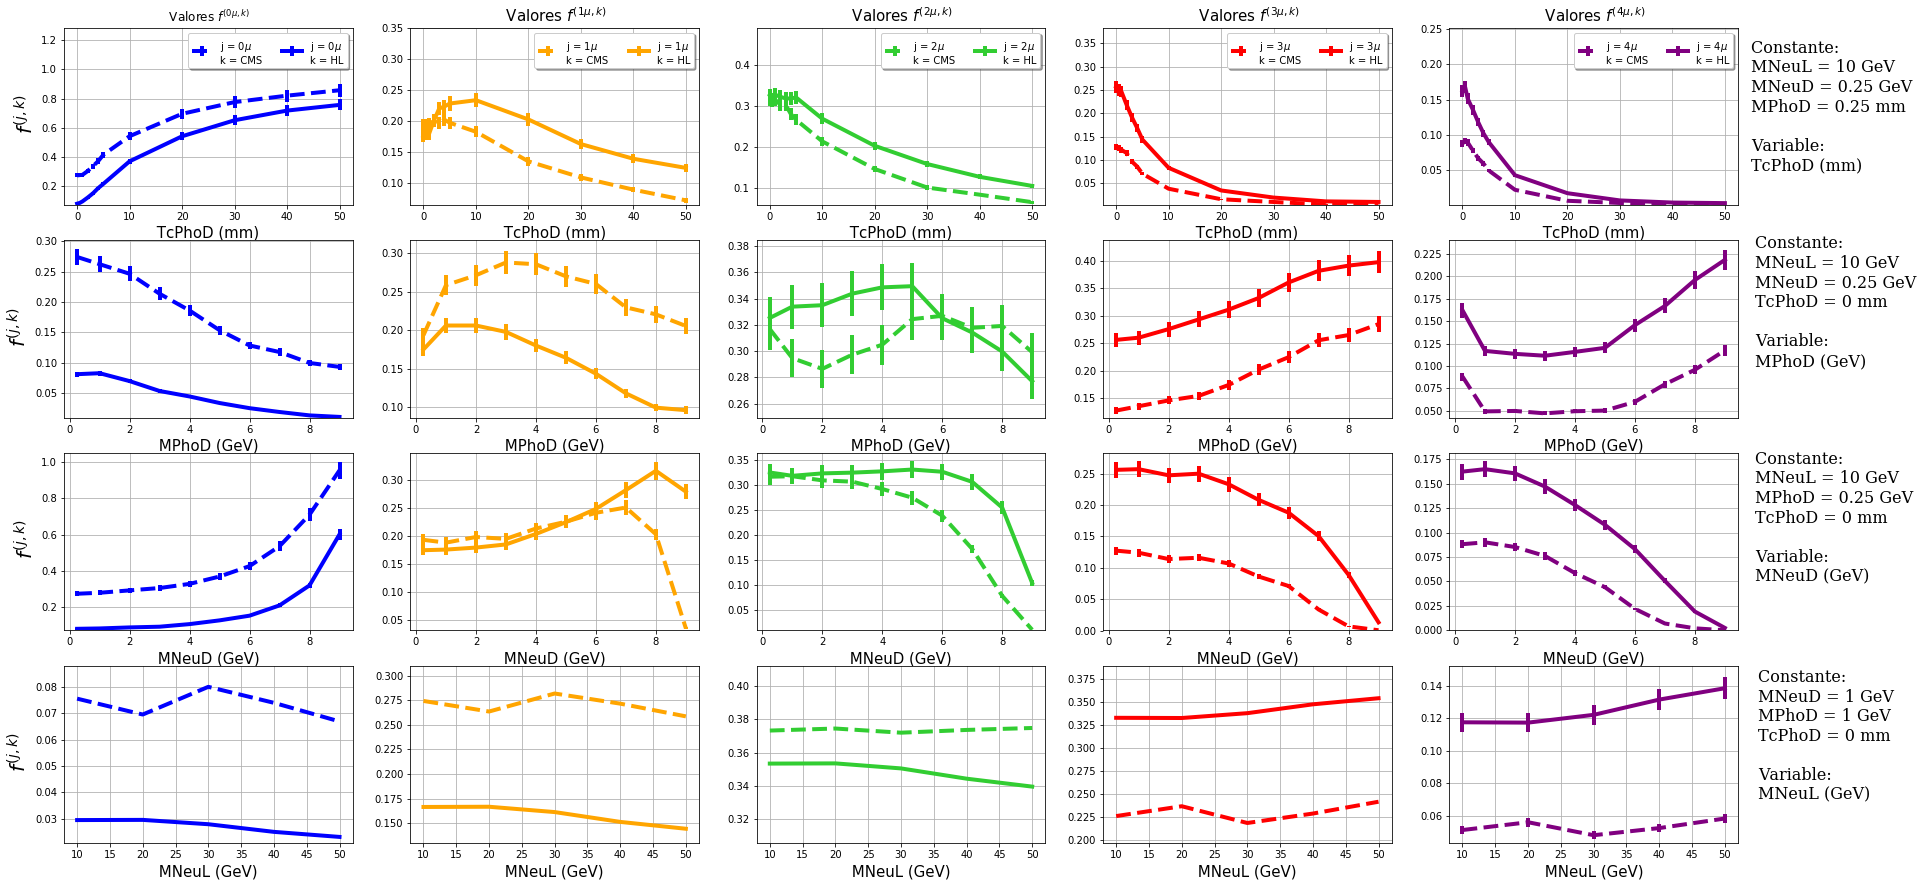
\includegraphics[width=1.2\textwidth]{Simulacion/imagenes/Comparacion_Distribucion_Entries.png}
%\caption{Distribuciones de frecuencia de las entradas $f^{(j,~k)}$ ante cambios de \texttt{MNeuD}.}
%\label{entradasALL}
%
%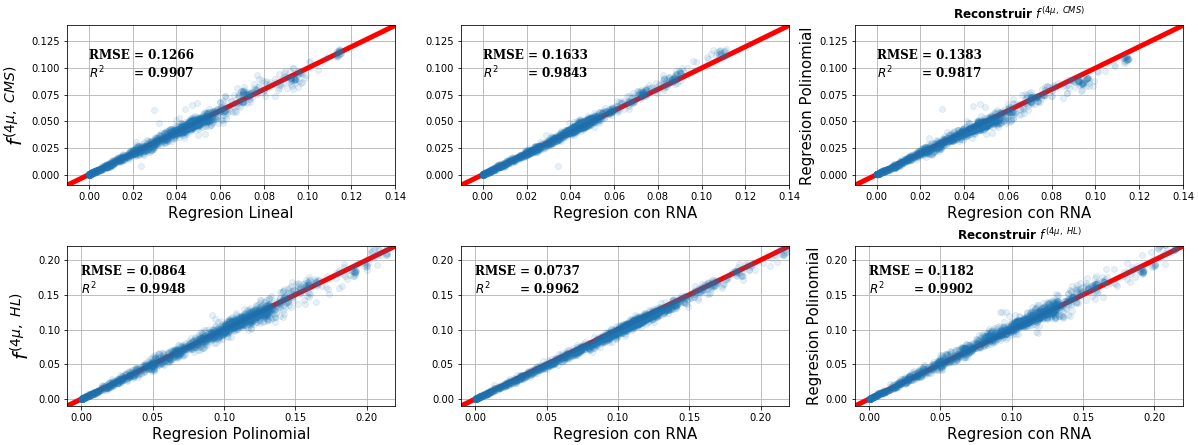
\includegraphics[width=1\textwidth]{Simulacion/imagenes/ML_Entries.png}
%\caption{Resultados de la regresión de los valores de frecuencia $f^{(4\mu,~k)}$.}
%\label{regresionALL}
%\end{figure}
%\end{landscape} 








